\documentclass{sig-alternate-10}


\usepackage{tikz}
\usepackage{forest}
\usepackage{framed}
\usepackage{cancel}
\usepackage{enumerate}

\newtheorem{demo}{Example}[section]

\newcommand{\textliteral}[1]{\textup{\texttt{"#1"}}}
\newcommand{\keyword}[1]{\textup{\textsf{#1}}}
\newcommand{\Opt}[1]{\keyword{Opt}\left\{#1\right\}}
\newcommand{\Seq}[1]{\keyword{Seq}\left\{#1\right\}}
\newcommand{\Rel}[1]{\keyword{Rel}\left\{#1\right\}}
\newcommand{\Ctx}[2]{\keyword{Ctx}_{#1}\left\{#2\right\}}
\newcommand{\Tuple}[1]{\langle #1 \rangle}
\newcommand{\Quotient}[2]{{#1}\Big/\raisebox{-1ex}{\!\small$#2$}}
\newcommand{\Void}{\keyword{Void}}
\newcommand{\Dept}{\keyword{Dept}}
\newcommand{\Emp}{\keyword{Emp}}
\newcommand{\Pos}{\keyword{Pos}}
\newcommand{\Text}{\keyword{Text}}
\newcommand{\Int}{\keyword{Int}}
\newcommand{\Bool}{\keyword{Bool}}
\newcommand{\Department}{\keyword{department}}
\newcommand{\Employee}{\keyword{employee}}
\newcommand{\Name}{\keyword{name}}
\newcommand{\Position}{\keyword{position}}
\newcommand{\Salary}{\keyword{salary}}
\newcommand{\Manager}{\keyword{manager}}
\newcommand{\Subordinate}{\keyword{subordinate}}
\newcommand{\TopSalary}{\keyword{top\_salary}}
\newcommand{\Level}{\keyword{level}}
\newcommand{\Null}{\keyword{null}}
\newcommand{\True}{\keyword{true}}
\newcommand{\False}{\keyword{false}}
\newcommand{\Here}{\keyword{here}}
\newcommand{\Length}{\keyword{length}}
\newcommand{\Count}{\keyword{count}}
\newcommand{\Exists}{\keyword{exists}}
\newcommand{\Any}{\keyword{any}}
\newcommand{\All}{\keyword{all}}
\newcommand{\Sum}{\keyword{sum}}
\newcommand{\Max}{\keyword{max}}
\newcommand{\Min}{\keyword{min}}
\newcommand{\Mean}{\keyword{mean}}
\newcommand{\Select}{\keyword{select}}
\newcommand{\Filter}{\keyword{filter}}
\newcommand{\Define}{\keyword{define}}
\newcommand{\Size}{\keyword{size}}
\newcommand{\Sort}{\keyword{sort}}
\newcommand{\Asc}{\keyword{asc}}
\newcommand{\Desc}{\keyword{desc}}
\newcommand{\Take}{\keyword{take}}
\newcommand{\Skip}{\keyword{skip}}
\newcommand{\Unique}{\keyword{unique}}
\newcommand{\Connect}{\keyword{connect}}
\newcommand{\Group}{\keyword{group}}
\newcommand{\Rollup}{\keyword{rollup}}
\newcommand{\Before}{\keyword{before}}
\newcommand{\Around}{\keyword{around}}
\newcommand{\Given}{\keyword{given}}
\newcommand{\To}{\boldsymbol{.}}
\newcommand{\Apply}{\!\boldsymbol{:}\!}
\newcommand{\As}{\Rightarrow}

\usetikzlibrary{arrows,arrows.meta,positioning}

\tikzset{
    entity diagram/.style={
        > = stealth',
        shorten > = 1pt,
        node distance = 2cm and 2.5cm,
        set/.style = {
            draw, rectangle, thick, font=\sffamily,
            minimum width=1.5cm, minimum height=.75cm,
            text height=1.5ex, text depth=.25ex},
        map/.style = {font=\small\sffamily}
    }
}

\tikzset{
    traverse/.style={
        ->,
        > = stealth',
        shorten < = 2pt,
        shorten > = 2pt
    }
}

\forestset{
    unfolded database/.style={
        void/.style = {
            draw, circle,
        },
        map/.style = {
            draw, rectangle, rounded corners=1mm,
            minimum width=2cm, minimum height=.5cm,
            text height=1.5ex, text depth=.25ex,
            font=\small\sffamily},
        box/.style = {
            draw, rectangle, rounded corners=1mm,
            minimum width=2cm, minimum height=.5cm,
            font=\small\sffamily},
        more/.style = {
            rectangle, minimum height=.5cm,
            edge path = {
                \noexpand
                \path [draw, -] (!u.parent anchor) -- +(0.15cm,0);
                \noexpand
                \path [draw, -, densely dotted] (!u.parent anchor) ++(0.15cm,0) -- +(0.15cm,0);
                \noexpand
                \path [draw, -] (!u.parent anchor) ++(0.1cm,0) -- +(0,-0.05cm);
                \noexpand
                \path [draw, -, densely dotted] (!u.parent anchor) ++(0.1cm,-0.05cm) -- +(0,-0.2cm);
            },
            l sep=0
        },
        and more/.style = {
            edge path = {
                \noexpand
                \path [\forestoption{edge}] (!u.parent anchor) -- +(0.1cm,0) |- (.child anchor);
                \noexpand
                \path [\forestoption{edge}] (!u.parent anchor |- .child anchor) ++(0.1cm,0) -- +(0,-0.05cm);
                \noexpand
                \path [draw, -, densely dotted] (!u.parent anchor |- .child anchor) ++(0.1cm,-0.05cm) -- +(0,-0.2cm);
            }
        },
        singular/.style = {
            edge={-}},
        optional/.style = {
            edge={-{Circle[open,length=3.5pt]}}},
        plural/.style = {
            edge={-{Straight Barb[reversed,length=3.5pt]}, shorten >=-0.5pt}},
        selected/.style = { thick, fill=lightgray!25 },
        selected edge/.style = { edge={thick} },
        for tree = {
            grow'=0,
            child anchor=west,
            parent anchor=east,
            anchor=west,
            calign=first,
            edge path={
                \noexpand
                \path [\forestoption{edge}] (!u.parent anchor) -- +(0.1cm,0) |- (.child anchor);
            },
        }
    }
}



\def\sharedaffiliation{\end{tabular}\newline\begin{tabular}{c}}

\begin{document}

\title{Query Combinators}

\numberofauthors{2}
\author{
    \alignauthor Clark C. Evans \\ \email{cce@clarkevans.com}
    \alignauthor Kyrylo Simonov \\ \email{xi@resolvent.net}
    \sharedaffiliation
    \affaddr{Prometheus Research, LLC} \\
}

%\begin{CCSXML}
%<ccs2012>
%<concept>
%<concept_id>10002951.10002952.10003197</concept_id>
%<concept_desc>Information systems~Query languages</concept_desc>
%<concept_significance>500</concept_significance>
%</concept>
%<concept>
%<concept_id>10002951.10002952.10002953</concept_id>
%<concept_desc>Information systems~Database design and models</concept_desc>
%<concept_significance>300</concept_significance>
%</concept>
%<concept>
%<concept_id>10003752.10010124.10010131.10010133</concept_id>
%<concept_desc>Theory of computation~Denotational semantics</concept_desc>
%<concept_significance>300</concept_significance>
%</concept>
%</ccs2012>
%\end{CCSXML}

%\ccsdesc[500]{Information systems~Query languages}
%\ccsdesc[300]{Information systems~Database design and models}
%\ccsdesc[300]{Theory of computation~Denotational semantics}

\maketitle


\begin{abstract}
    We introduce Rabbit, a combinator-based database query language.  It is
    designed for data analysts and other accidental programmers to let them
    query complex structured data.

    Rabbit features a novel semantics of a database query and query
    composition.  A query is represented as a mapping with certain input type,
    output type and cardinality.  Notably, query cardinality is modeled as a
    monadic wrapper over its output type, which is what makes Rabbit queries
    highly composable and let it express common data operations as \emph{query
    combinators}.  In particular, monadic composition becomes a data traversal
    combinator.  Other combinators express operations for aggregating,
    filtering, grouping, sorting and paginating data, cube operations and
    operations on self-referential data.  By extending the query model with a
    comonadic wrapper over its input type, we can express queries with running
    aggregates and parametric queries.  Aside from semantics, Rabbit features
    pipeline syntax notation, which permits and stimulates the users to
    construct database queries as a series of distinct steps, each individually
    crafted and tested.  We believe that for data analytics, Rabbit presents a
    viable alternative to SQL.
\end{abstract}



\section{Introduction}
\label{sec:introduction}

\emph{Combinator pattern} is a well-known technique for designing declarative
domain-specific languages (DSLs). This technique views a DSL as an algebra of
self-con\-tained processing blocks, which either come from a set of predefined
atomic \emph{primitives} or are constructed from other blocks using block
operators (combinators).  Using the combinator pattern, a DSL is specified by:
the interface of its processing blocks, a set of primitives, and a collection
of combinators.

The combinator pattern gives us a roadmap to design a database query language:

\begin{enumerate}
\item
Define the interface of a database query.
\item
Describe the set of primitive queries.
\item
Describe combinators for making composite queries.
\end{enumerate}

To elaborate on this idea and to demonstrate example queries, we need some
sample structured data.  Throughout this paper, we use a simple database that
contains just two classes of entities: \emph{departments} and \emph{employees}.
Each department entity has one attribute: \emph{name}.
Each employee entity has three attributes: \emph{name}, \emph{position} and
\emph{salary}.
Each employee belongs to a department.
An employee may have a \emph{manager}, who is also an employee.

The structure of this database can be visualized as a directed graph, where entity
classes and attribute types become graph nodes, while attributes and relationships
become arcs (see Figure~\ref{fig:sample-schema}).  This diagram
suggests presentation of the database in terms of types and functions.
Namely, graph arcs represent functions that store data about attributes and
relationships, such as
\begin{alignat*}{3}
    & \Department && : \Emp && \to \Dept, \\
    & \Name && : \Dept && \to \Text.
\end{alignat*}
This is known as the functional database model (\cite{Kerschberg1976}).

\begin{figure}
    \label{fig:sample-schema}
    \centering
    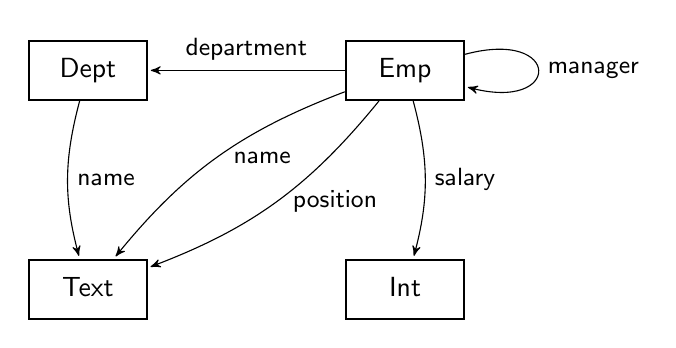
\begin{tikzpicture}
        [
            > = stealth',
            shorten > = 1pt,
            node distance = 2cm and 2.5cm,
            set/.style = {
                draw, rectangle, thick, font=\sffamily,
                minimum width=1.5cm, minimum height=.75cm,
                text height=1.5ex, text depth=.25ex},
            map/.style = {font=\small\sffamily}
        ]
        \node [set] (Dept) {Dept};
        \node [set] (Emp) [right=of Dept] {Emp};
        \node [set] (Text) [below=of Dept] {Text};
        \node [set] (Int) [below=of Emp] {Int};
        \draw [->] (Dept) to [bend right=15] node [map, right] {name} (Text);
        \draw [->] (Emp) to [bend right=15] node [map, right] {\;name} (Text);
        \draw [->] (Emp) to [bend left=15] node [map, right] {\;position} (Text);
        \draw [->] (Emp) to [bend left=15] node [map, right] {salary} (Int);
        \draw [->] (Emp) to node [map, above] {department} (Dept);
        \draw [->] (Emp) to [loop right] node [map, right] {manager} (Emp);
    \end{tikzpicture}
    \caption{Sample database schema}
\end{figure}

This model provides us with a starting point on our combinator pattern roadmap.
Any function on an entity set could be seen as a database query.  Then, all the
attributes and relationships form a set of primitive queries.  Composition of
functions becomes a binary query combinator.  With these considerations, we can
write our first composite query.

\begin{example}
    Given an employee entity, show the name of their department.
    \begin{equation*}
        \Department{.}\Name: \Emp \to \Text
    \end{equation*}
\end{example}

In this example, $\Department{.}\Name$ is a query written in Rabbit notation,
$\Emp \to \Text$ is its signature.  The period $({.})$ denotes the composition
combinator, which is a polymorphic binary operator with signature
\begin{equation*}
        (-{.}-) : (A \to B) \times (B \to C) \to (A \to C).
\end{equation*}

Even though we got a query interface, a set of primitives and one query
combinator, it doesn't yet feel like a proper query language.  Let us discuss
what is missing.

First, it is awkward that the query interface always demands an input.  It
means that we cannot express an input-free query like \emph{show a list of all
departments}.

Further, relationships between entities got a direction arbitrarily assigned to
them.  Indeed, we chose to encode the relationship between departments and
employees as a primitive with input $\Emp$ and output $\Dept$.  But this
relationship is symmetric and we may just as well be interested in finding,
\emph{for any given department, the corresponding set of employees}.  This
query cannot be encoded as a function because its signature $\Dept \to \Emp$
would incorrectly imply that there is exactly one employee per department.  The
query interface is unable to express multivalued or \emph{plural}
relationships.

The interface also fails to capture the semantics of \emph{optional} attributes
and relationships.  Such is the relationship between employees and their
managers, which, according to Figure~\ref{fig:sample-schema}, is encoded by
a primitive with signature $\Emp \to \Emp$.
But this signature implies that every employee must have a manager, which is
untrue.  Apparently, pure functional interface is too restrictive to express
the variety of relationships between database entities.

To improve this sketch of a query language, we will extend the query interface
to support optional and plural values, add primitives to express entity classes
and inverse relationships and implement common data operations in a
comprehensive library of query combinators.

This paper is organized as follows.

In Section~\ref{sec:cardinality}, we introduce query cardinality as a mo\-nadic
wrapper over its output type, which will allow us to complete our set of
primitive queries.  We also show how any database can be unfolded to the
hierarchical form.

In Section~3, we define and demonstrate how to use combinators for data
traversal, aggregation, filtering, sorting and pagination.

In Section~4, we introduce combinators for exploring hierarchical
relationships.

In Section~5, we define quotient types and show how to use them for grouping
and cube operations.

In Section~6, we show how to extend the query interface with comonadic wrapper
over its input type to support context-aware combinators.  This gives us
ability to express queries with running aggregates and parametric queries.

In Section~7, we formally describe the query interface and the composition
combinator.

In Section~8, we briefly discuss some related work.



\section{Query Cardinality}
\label{sec:cardinality}

\begin{figure*}
    \label{fig:hierarchical-form}
    \centering
    \begin{forest}
        void/.style = {
            draw, circle},
        map/.style = {
            draw, rectangle, rounded corners=2mm,
            minimum width=1.5cm, minimum height=.5cm,
            text height=1.5ex, text depth=.25ex,
            font=\small\sffamily},
        blank/.style = {
            no edge},
        more/.style = {
            rectangle, minimum height=.5cm,
            edge={-{stealth'}}},
        singular/.style = {
            edge={-}},
        optional/.style = {
            edge={-{Circle[open,length=3.5pt]}}},
        plural/.style = {
            edge={-{Straight Barb[reversed,length=3.5pt]}, shorten >=-0.3pt}},
        for tree = {
            parent anchor=south,
            child anchor=north,
            edge path={
                \noexpand\path[\forestoption{edge}](!u.parent anchor) -- +(0,-4pt) -| (.child anchor)\forestoption{edge label};}}
        [{},void
            [department,map,plural
                [name,map,singular]
                [employee,map,plural
                    [name,map,singular]
                    [\dots,blank]
                    [department,map,singular
                        [\dots,more]
                        [\dots,more]]
                    [\dots,blank]
                    [subordinate,map,plural
                        [\dots,more]
                        [\dots,blank]
                        [\dots,more]]]]
            [employee,map,plural
                [name,map,singular]
                [position,map,singular]
                [salary,map,singular]
                [department,map,singular
                    [name,map,singular]
                    [employee,map,plural
                        [\dots,more]
                        [\dots,blank]
                        [\dots,more]]]
                [manager,map,optional
                    [\dots,more]
                    [\dots,blank]
                    [\dots,more]]
                [subordinate,map,plural
                    [\dots,more]
                    [\dots,blank]
                    [\dots,more]]]]
    \end{forest}
    \caption{Database schema in hierarchical form}
\end{figure*}

In Section~\ref{sec:introduction}, we suggested that any function defined on an
entity set can be seen as a query.  However, this query model failed to
represent optional and plural relationships as well as queries without apparent
input.  In this section, we resolve these issues by introducing the notion of
\emph{query cardinality}.

We found it difficult to model these two relationships:

\begin{enumerate}[(i)]
\item \label{itm:employee-to-manager}
\emph{An employee may report to another employee, the manager.}

\item \label{itm:department-to-employee}
\emph{Any department has a number of associated employees.}
\end{enumerate}

We were also puzzled on how to express input-free queries such as:

\begin{enumerate}[(i)]
\setcounter{enumi}{2}
\item \label{itm:department-set}
\emph{Show a list of all departments.}
\end{enumerate}

Let us start with relationships~(\ref{itm:employee-to-manager})
and~(\ref{itm:department-to-employee}).  Expressing them as queries with
signatures
\begin{equation*}
    \Emp \to \Emp, \qquad \Dept \to \Emp
\end{equation*}
would imply exactly one output value for any input.  But an employee may have
no manager, and a department may have more than one employee.

In programming practice, optional and plural values are stored using container
types.  So let us define two parametric types: $\Opt{A}$ as a zero or one value
of type $A$ and $\Seq{A}$ as a type of finite $A$-valued sequences, that is
\begin{equation*}
\Opt{A} = \{\bot\} \sqcup A, \qquad
\Seq{A} = \{[\;]\} \sqcup A \sqcup A^2 \sqcup \ldots.
\end{equation*}

With these, we can express relationships~(\ref{itm:employee-to-manager})
and~(\ref{itm:department-to-employee}) as primitives
\begin{alignat*}{3}
    & \Manager && : \Emp && \to \Opt{\Emp}, \\
    & \Employee && : \Dept && \to \Seq{\Emp}.
\end{alignat*}
The container structure over the query output is what we call the query
cardinality.

We can now guess the output type and cardinality of
query~(\ref{itm:department-set}).  Indeed, \emph{a list of all departments}
can only mean $\Seq{\Dept}$.

To describe the input this query, we need to introduce a \emph{singleton} type
\begin{equation*}
    \Void = \{\top\}.
\end{equation*}
Type $\Void$ has a unique inhabitant, and because there is no freedom in
choosing a value of this type, it can designate input that can never affect the
result of a query.  Thus, we can express~(\ref{itm:department-set}) with a
\emph{class} primitive
\begin{equation*}
    \Department : \Void \to \Seq{\Dept}
\end{equation*}
that produces all department entities.

Unfortunately, although containers let us represent optional and plural values,
they do not compose well.  For example, it is tempting to express a query that
\emph{for a given employee, finds their manager's salary} as a composition
\begin{equation} \label{eq:manager-to-salary}
    \Manager\To\Salary,
\end{equation}
or a query that \emph{shows the names of all departments} as
\begin{equation} \label{eq:department-to-name}
    \Department\To\Name.
\end{equation}
However, if we look at the signatures of the components
\begin{alignat*}{6}
    & \Manager && : \Emp && \to \Opt{\Emp}, \quad && \Salary && : \Emp && \to \Int, \\
    & \Department && : \Void && \to \Seq{\Dept}, \quad && \Name && : \Dept && \to \Text,
\end{alignat*}
we see that their intermediate domains do not agree, which means their
compositions are ill-formed.

To compose functions that carry extra structure with their output, we use a
concept of \emph{monadic composition} (\cite{Moggi1991}).

A monad is a parametric type $M\{A\}$ equipped with a generic function
$\operatorname{unit}_{M\{A\}} : A \to M\{A\}$ and a so-called monadic
composition rule that satisfy certain coherence axioms.  Monadic
composition of two functions
\begin{equation*}
    p : A \to M\{B\}, \qquad q : B \to M\{C\},
\end{equation*}
gives a function $p\,\To\,q$ with a signature of the same shape
\begin{equation*}
    p\,\To\,q : A \to M\{C\}.
\end{equation*}

Both $\Opt{A}$ and $\Seq{A}$ are monads.  Let us confirm that they admit
monadic composition.

Monadic composition of
\begin{equation*}
    p : A \to \Opt{B}, \qquad q : B \to \Opt{C}.
\end{equation*}
is just a composition of partial functions
\begin{equation*}
    p\,\To\,q : a \longmapsto \begin{cases}
        \bot & (p(a)=\bot\text{ or }q(p(a))=\bot), \\
        q(p(a)) & (\text{otherwise}).
    \end{cases}
\end{equation*}

To compose two sequence-valued functions
\begin{equation*}
    p : A \to \Seq{B}, \qquad q : B \to \Seq{C},
\end{equation*}
we first evaluate $p$ on the input $a$ of type $A$
\begin{equation*}
    a \overset{p}{\longmapsto} [b_1, b_2, \ldots],
\end{equation*}
then apply $q$ to every element of $p(a)$
\begin{equation*}
    [b_1, b_2, \ldots]
    \overset{[q]}{\longmapsto}
    [[c^{1}_{1}, c^{1}_{2}, \ldots], [c^{2}_{1}, c^{2}_{2}, \ldots], \ldots],
\end{equation*}
and finally erase the nested brackets
\begin{equation*}
    [[c^{1}_{1}, c^{1}_{2}, \ldots], [c^{2}_{1}, c^{2}_{2}, \ldots], \ldots]
    \overset{\cancel{\,[\;]\,}}{\longmapsto}
    [c^{1}_{1}, c^{1}_{2}, \ldots, c^{2}_{1}, c^{2}_{2}, \ldots].
\end{equation*}
The result is the value $(p\,\To\,q)(a)$ of type $\Seq{C}$.

Monadic (and regular) composition rules give us a way to compose queries of the
same cardinality.  To compose queries with mixed cardinalities, we promote
their cardinalities to a smallest common monadic container using a chain of
natural embeddings
\begin{equation*}
    A \hookrightarrow \Opt{A} \hookrightarrow \Seq{A}.
\end{equation*}
These embeddings are defined by
\begin{alignat*}{5}
    & \; && \bot && : \Opt{A} && \longmapsto [\;] && : \Seq{A}, \\
    & a : A \longmapsto\ && a && : \Opt{A} && \longmapsto [a] && : \Seq{A}.
\end{alignat*}

We can now state the query composition rule as follows: find the largest
cardinality of the components; lift all components to this cardinality; use
monadic composition.  For example, this rule gives queries
(\ref{eq:manager-to-salary}) and (\ref{eq:department-to-name}) signatures
\begin{alignat*}{3}
    & \Manager\To\Salary && : \Emp && \to \Opt{\Text}, \\
    & \Department\To\Name && : \Void && \to \Seq{\Int}.
\end{alignat*}

We are ready to present the design of a combinator-based query language.

\begin{description}
\item[Query interface:]
A database query is a function of the form
\begin{equation*}
    p : A \to M\{B\}.
\end{equation*}
We call $A$ its input type, $B$ its output type, and $M$ its monadic
cardinality.  $M\{B\}$ could be one of $B$, $\Opt{B}$ or $\Seq{B}$ and
the respective queries are called singular, optional or plural.

\item[Primitives:]
The set of primitives include class primitives
\begin{alignat*}{3}
    & \Department && : \Void && \to \Seq{\Dept}, \\
    & \Employee && : \Void && \to \Seq{\Dept},
\end{alignat*}
attributes
\begin{alignat*}{6}
    & \Name && : \Dept && \to \Text, \qquad
    && \Name && : \Emp && \to \Text, \\
    & \Position && : \Emp && \to \Text, \qquad
    && \Salary && : \Emp && \to \Int,
\end{alignat*}
and relationships
\begin{alignat*}{3}
    & \Department && : \Emp && \to \Dept, \\
    & \Employee && : \Dept && \to \Seq{\Emp}, \\
    & \Manager && : \Emp && \to \Opt{\Emp}, \\
    & \Subordinate && : \Emp && \to \Seq{\Emp}.
\end{alignat*}
Note that we allow multiple primitives to share the same name as long as they
do not share the same input.

\item[Combinators:]
Binary composition combinator takes two queries
\begin{equation*}
    p : A \to M_1\{B\}, \qquad
    q : B \to M_2\{C\}
\end{equation*}
and produces a query of the form
\begin{equation*}
    p\,\To\,q : A \to M\{C\}.
\end{equation*}
Here, $M = M_1 \lor M_2$ is the smallest common cardinality of $M_1$ and $M_2$.

More combinators will be described in the next section.
\end{description}

To visualize the full set of primitives, we could alter
Figure~\ref{fig:sample-schema} to add the $\Void$ node and missing arcs.  But
instead, we prefer to unfold it into an infinite tree, where each node stands
for a primitive and any two adjacent nodes are composable primitives (see
Figure~\ref{fig:hierarchical-form}).  We can say that
Figure~\ref{fig:hierarchical-form} represents the database in hierarchical
database model, which suggests us another model of a database query: a
transformation of a hierarchical database.



\section{Query Combinators}
\label{sec:combinators}

In this section, we show how the query model defined in
Section~\ref{sec:cardinality} can support a wide range of operations on data.

\subsection*{Extracting Data}

By traversing the tree of Figure~\ref{fig:unfolded-form}, we can extract data
from the database.

\begin{demo}
    \label{ex:department-name}
    Show the name of each department.
    \begin{equation*}
        \Department\To\Name
    \end{equation*}
\end{demo}

This example is constructed by descending through nodes $\Department$ and
$\Name$, which represent primitives
\begin{alignat*}{3}
    & \Department && : \Void && \to \Seq{\Dept}, \\
    & \Name && : \Dept && \to \Text.
\end{alignat*}
The composition of the primitives inherits the input of the first component and
the output of the second component.  Since one of the components is plural, the
composition is also plural, which gives it a signature
\begin{equation*}
    \Department\To\Name : \Void \to \Seq{\Text}.
\end{equation*}

\begin{demo}
    \label{ex:department-employee-name}
    For each department, show the name of each employee.
    \begin{equation*}
        \Department\To\Employee\To\Name
    \end{equation*}
\end{demo}

This example takes a path through
\begin{alignat*}{3}
    & \Department && : \Void && \to \Seq{\Dept}, \\
    & \Employee && : \Dept && \to \Seq{\Emp}, \\
    & \Name && : \Emp && \to \Text,
\end{alignat*}
to construct a query
\begin{equation*}
    \Department\To\Employee\To\Name : \Void \to \Seq{\Text}.
\end{equation*}

This query produces a list of employee names.  Since each employee belongs to
exactly one department, the list should contain the name of every employee.
The order in which the names appear in the output depends on the intrinsic
order of the $\Department$ and $\Employee$ primitives, but, in any case,
employees within the same department will be coupled together.

The same collection of names, although not necessarily in the same order, is
produced by the following example.

\begin{demo}
    \label{ex:employee-name}
    Show the name of each employee.
    \begin{equation*}
        \Employee\To\Name
    \end{equation*}
\end{demo}

On the other hand, the next example is very different from the apparently
similar Example~\ref{ex:department-name}.

\begin{demo}
    \label{ex:employee-department-name}
    For each employee, show the name of their department.
    \begin{equation*}
        \Employee\To\Department\To\Name
    \end{equation*}
\end{demo}

Here, we should see a list of department names, but each name will appear as
many times as there are employees in the corresponding department.

\begin{demo}
    \label{ex:employee-position}
    Show the position of each employee.
    \begin{equation*}
        \Employee\To\Position
    \end{equation*}
\end{demo}

Similarly, $\Employee\To\Position$ will output duplicate position titles.  We
will see how to produce a list of \emph{unique} positions in
Section~\ref{sec:quotients}.

\begin{demo}
    \label{ex:employee}
    Show all employees.
    \begin{equation*}
        \Employee
    \end{equation*}
\end{demo}

This example emits a sequence of employee entities, which, in practice, could
be represented as records with employee attributes.


\begin{table}
    \begin{framed}
    \textbf{Identity and constants}
    \begin{alignat*}{3}
        & \Here && : A \to A && = a \mapsto a \\
        & 150000 && : A \to \Int && = a \mapsto 150000 \\
        & \Home && : A \to \Void && = a \mapsto \top \\
        & \Null && : A \to \Opt{B} && = a \mapsto \bot
    \end{alignat*}
    \textbf{Some scalar combinators}
    \begin{alignat*}{3}
        & {=},{\ne} && : (A \to B, A \to B) && \to (A \to \Bool) \\
        & {<},{\le},{>},{\ge} && : (A \to B, A \to B) && \to (A \to \Bool) \\
        & {\&},{|} && : (A \to \Bool, A \to \Bool) && \to (A \to \Bool) \\
        & {+},{-} && : (A \to \Int, A \to \Int) && \to (A \to \Int) \\
        & \Length && : (A \to \Text) && \to (A \to \Int)
    \end{alignat*}
    \textbf{Aggregate combinators}
    \begin{alignat*}{3}
        & \Count && : (A \to \Seq{B}) && \to (A \to \Int) \\
        & \Exists && : (A \to \Seq{B}) && \to (A \to \Bool) \\
        & \Any, \All && : (A \to \Seq{\Bool}) && \to (A \to \Bool) \\
        & \Sum && : (A \to \Seq{\Int}) && \to (A \to \Int) \\
        & \Max, \Min && : (A \to \Seq{\Int}) && \to (A \to \Opt{\Int})
    \end{alignat*}
    \textbf{Sequence transformers}
    \begin{alignat*}{4}
        & \Filter && : (&& A \to \Seq{B}, B \to \Bool) && \to (A \to \Seq{B}) \\
        & \Sort && : (&& A \to \Seq{B}, && \\
        & && && B \to C_1, \ldots, B \to C_n) && \to (A \to \Seq{B}) \\
        & \Take && : (&& A \to \Seq{B}, A \to \Int) && \to (A \to \Seq{B}) \\
        & \Unique : (A \to \Seq{B})\hidewidth && && && \to (A \to \Seq{B})
    \end{alignat*}
    \textbf{Selector and modifiers}
    \begin{alignat*}{2}
        & \Select & : (& A \to \Wrap{M}{B}, \\
        & && B \to \Wrap{M_1}{C_1}, \ldots, B \to \Wrap{M_n}{C_n}) \\
        & \;\to (A \to \Wrap{M}{\Tuple{\Wrap{M_1}{C_1}, \ldots, \Wrap{M_n}{C_n}}})\hidewidth && \\
        & \Define & : (& A \to \Wrap{M}{B}, B \to T) \to (A \to \Wrap{M}{B}) \\
        & \Asc, \Desc & : (& A \to B) \to (A \to B_\lessgtr)
    \end{alignat*}
    \textbf{Hierarchical connector}
    \begin{equation*}
        \Connect : (A \to \Opt{A}) \to (A \to \Seq{A})
    \end{equation*}
    \textbf{Grouping}
    \begin{alignat*}{2}
        & \Group && : ( A \to \Seq{B}, B \to C_1, \ldots, B \to C_n) \\
        & \;\to (A && \to \Seq{\Tuple{C_1, \ldots, C_n, \Seq{B}}}) \\
        & \Rollup && : ( A \to \Seq{B}, B \to C_1, \ldots, B \to C_n) \\
        & \;\to (A && \to \Seq{\Tuple{\Opt{C_1}, \ldots, \Opt{C_n}, \Seq{B}}})
    \end{alignat*}
    \textbf{Context primitives and combinators}
    \begin{align*}
        & \Frame : (\Rel{A} \to \Wrap{M}{B}) \to (A \to \Wrap{M}{B}) \\
        & \Before, \Around : \Rel{A} \to \Seq{A} \\
        & \Given : (\Env{T}{A} \!\to\! \Wrap{M}{B}, A \!\to\! T) \to (A \!\to\! \Wrap{M}{B}) \\
        & \textit{\textsf{PARAM}} : \Env{T}{A} \to T
    \end{align*}
    \vspace*{-\bigskipamount}
    \end{framed}
    \caption{Some primitives and combinators}
    \label{tab:common-combinators}
\end{table}



\subsection*{Summarizing Data}

Let us show how the extracted data can be summarized.

\begin{demo}
    \label{ex:count-department}
    Show the number of departments.
    \begin{equation*}
        \Count(\Department)
    \end{equation*}
\end{demo}

This query produces a single number, so that its signature is
\begin{equation*}
    \Count(\Department) : \Void \to \Int.
\end{equation*}
It is constructed by applying the $\Count$ combinator to a query that generates
\emph{a list of all departments}
\begin{equation*}
    \Department : \Void \to \Seq{\Dept}.
\end{equation*}
Comparing the signatures of these two queries, we can derive the signature of
the $\Count$ combinator, in this specific case
\begin{equation*}
    (\Void \to \Seq{\Dept}) \to (\Void \to \Int),
\end{equation*}
and, in general
\begin{equation*}
    \Count: (A \to \Seq{B}) \to (A \to \Int).
\end{equation*}
In other words, the $\Count$ combinator transforms any sequence-valued query
to an integer-valued query.  It is implemented by lifting the function that
computes the length of a sequence
\begin{equation*}
    |-| : \Seq{A} \to \Int
\end{equation*}
to a query combinator
\begin{equation*}
    \Count(q) = a \mapsto |q(a)|.
\end{equation*}

We call $\Count$ and other unary combinators that transform a plural query to a
singular (or optional) query \emph{aggregate} combinators.

The next example follows the same pattern.

\begin{demo}
    \label{ex:max-employee-salary}
    Show the highest salary of all employees.
    \begin{equation*}
        \Max(\Employee\To\Salary)
    \end{equation*}
\end{demo}

It extracts the relevant data with
\begin{equation*}
    \Employee\To\Salary : \Void \to \Seq{\Int}
\end{equation*}
and summarizes it using the $\Max$ aggregate
\begin{equation*}
    \Max(\Employee\To\Salary) : \Void \to \Opt{\Int}.
\end{equation*}
This query is optional since it produces no output when the database contains
no employees.

\begin{demo}
    \label{ex:department-count-employee}
    Show the number of employees in each department.
    \begin{equation*}
        \Department\To\Count(\Employee)
    \end{equation*}
\end{demo}

In this example, we transform a plural relationship, \emph{all employees in the
given department}
\begin{equation*}
    \Employee : \Dept \to \Seq{\Emp}
\end{equation*}
to a calculated attribute, \emph{the number of employees in the given
department}
\begin{equation*}
    \Count(\Employee) : \Dept \to \Int.
\end{equation*}
Then we attach it to
\begin{equation*}
    \Department : \Void \to \Seq{\Dept}
\end{equation*}
to get \emph{the number of employees in each department}
\begin{equation*}
    \Department\To\Count(\Employee) : \Void \to \Seq{\Int}.
\end{equation*}

Using the combinator $\Max$, we can further collapse this list to a single
number, as shown in the next example.

\begin{demo}
    \label{ex:max-department-count-employee}
    Show the size of the largest department.
    \begin{equation*}
        \Max(\Department\To\Count(\Employee))
    \end{equation*}
\end{demo}

\subsection*{Pipeline Notation}

Queries are often constructed incrementally, by extracting relevant data and
then shaping it into the desired form with a chain of combinators.  This
construction is made apparent with the \emph{pipeline notation}.

In pipeline notation, the first argument of a combinator is placed in front of
it, separated by colon (``$\,\Apply\,$''):
\begin{equation*}
    p \Apply F \equiv F(p), \qquad
    p \Apply F(q_1,\ldots,q_n) \equiv F(p,q_1,\ldots,q_n).
\end{equation*}
For example, $\Count(\Department)$ could also be written
\begin{equation*}
    \Department\Apply\Count.
\end{equation*}

A more sophisticated query written in pipeline notation is shown in the
following example.

\begin{demo}
    \label{ex:top-ten-highest-paid-policemen}
    Show the top 10 highest paid employees in the Police department.
    \begin{align*}
        & \Employee \\
        & \Apply\Filter(\Department\To\Name = \textliteral{POLICE}) \\
        & \Apply\Sort(\Salary\Apply\Desc) \\
        & \Apply\Select(\Name,\; \Position,\; \Salary) \\
        & \Apply\Take(10)
    \end{align*}
\end{demo}

Without pipeline notation, this query is much less intelligible:
\begin{multline*}
    \Take(\Select(\Sort(\Filter( \\
    \Employee,\; \Department\To\Name = \textliteral{POLICE}), \\
    \Desc(\Salary)),\; \Name,\; \Position,\; \Salary),\; 10).
\end{multline*}

Combinators $\Filter$, $\Sort$, $\Select$ and $\Take$ used in this query are
described below.

\subsection*{Filtering Data}

We can now demonstrate how to produce entities that satisfy a certain
condition.

\begin{demo}
    \label{ex:filter-by-salary}
    Which employees have a salary higher than \$150k?
    \begin{equation*}
        \Employee\Apply\Filter(\Salary>150000)
    \end{equation*}
\end{demo}

This query introduces several concepts.

First, the integer literal $150000$ represents a primitive query that
\emph{for any given employee, produces the number $150000$}
\begin{equation*}
    150000 : \Emp \to \Int = e \mapsto 150000.
\end{equation*}

Second, the relational symbol ${>}$ denotes a binary combinator, which builds a
query \emph{for a given employee, show whether their salary is higher than
\$150000}
\begin{equation*}
    \Salary > 150000 : \Emp \to \Bool.
\end{equation*}
The combinator
\begin{equation*}
    \placeholder>\placeholder : (A \to \Int,\; A \to \Int) \to (A \to \Bool)
\end{equation*}
is implemented by lifting the relational operator
\begin{equation*}
    \placeholder>\placeholder : (\Int,\; \Int) \to \Bool
\end{equation*}
to an operation on queries
\begin{equation*}
    (p > q) = a \mapsto (p(a) > q(a)).
\end{equation*}

Third, a binary combinator $\Filter$ emits those $\Employee$ entities that
satisfy the condition $\Salary > 150000$.  In general, given
\begin{equation*}
    p : A \to \Seq{B}, \qquad q : B \to \Bool,
\end{equation*}
a query
\begin{equation*}
    \Filter(p,\; q) : A \to \Seq{B}
\end{equation*}
produces the values of $p$ that satisfy condition $q$
\begin{equation*}
    \Filter(p,\; q) = a \mapsto [\,b \mid b \gets p(a),\; q(b)=\True\,].
\end{equation*}

The following example shows how $\Filter$ could be used with other combinators.

\begin{demo}
    \label{ex:filter-by-size-and-count}
    How many departments have more than 1000 employees?
    \begin{align*}
        & \Department \\
        & \Apply\Filter(\Count(\Employee)>1000) \\
        & \Apply\Count
    \end{align*}
\end{demo}

\subsection*{Sorting and Paginating Data}

The combinator $\Sort$, applied to a plural query, sorts the query output in
ascending order.

\begin{demo}
    \label{ex:sort-department-name}
    Show the names of all departments in alphabetical order.
    \begin{equation*}
        \Sort(\Department\To\Name)
    \end{equation*}
\end{demo}

The combinator $\Sort$ is implemented by lifting a sequence function
\begin{equation*}
    \Sort : \Seq{A} \to \Seq{A}
\end{equation*}
to a query combinator
\begin{align*}
    & \Sort : (A \to \Seq{B}) \to (A \to \Seq{B}), \\
    & \Sort(p) = a \mapsto \Sort(p(a)).
\end{align*}

\begin{demo}
    \label{ex:sort-employee-by-salary}
    Show all employees ordered by salary.
    \begin{equation*}
        \Employee\Apply\Sort(\Salary)
    \end{equation*}
\end{demo}

In this example, a list of employees is sorted by the value of the attribute
$\Salary$, which is supplied as a second argument to the $\Sort$ combinator.
In this form, $\Sort$ has a signature
\begin{equation*}
    \Sort : (A \to \Seq{B},\; B \to C) \to (A \to \Seq{B}).
\end{equation*}

\begin{demo}
    \label{ex:sort-employee-by-salary-desc}
    Show all employees ordered by salary, highest paid first.
    \begin{equation*}
        \Employee\Apply\Sort(\Salary\Apply\Desc)
    \end{equation*}
\end{demo}

Here, the sort key is wrapped with the combinator $\Desc$ to indicate the
descending sort order.

It is not immediately obvious how to implement $\Desc$ without violating the
query model.  Na\"{\i}vely, $\Desc$ acts like a negation operator, however, not
every type supports negation.  Instead, we make the sort order a part of the
type definition, so that
\begin{equation*}
    \Int_{\le} \quad\text{and}\quad \Int_{\ge}
\end{equation*}
could indicate the integer type with ascending and descending sort order
respectively.  Then, $\Desc$ could operate by switching the sort order of the
output type and be given a signature
\begin{equation*}
    \Desc : (A \to B) \to (A \to B_{\ge}).
\end{equation*}

\begin{demo}
    \label{ex:sort-employee-by-salary-take-top}
    Who are the top 1\% of highest paid employees?
    \begin{align*}
        & \Employee \\
        & \Apply\Sort(\Salary\Apply\Desc) \\
        & \Apply\Take(\Count(\Employee)\mathbin \div 100)
    \end{align*}
\end{demo}

In this example, only the first 1\% of employees are retained by the combinator
$\Take$, which has two arguments: a query that produces a sequence of employees
\begin{equation*}
    \Employee\Apply\Sort(\Salary\Apply\Desc) : \Void \to \Seq{\Emp}
\end{equation*}
and a query that returns how many employees to take
\begin{equation*}
    \Count(\Employee) \div 100 : \Void \to \Int.
\end{equation*}
Notice that both arguments of $\Take$ have the same input ($\Void$ in this
case), which is reflected in the signature
\begin{equation*}
    \Take : (A \to \Seq{B},\; A \to \Int) \to (A \to \Seq{B}).
\end{equation*}

\subsection*{Query Output}

The combinator $\Select$ customizes the query output.

Previously, we constructed a query to \emph{show the number of employees in
each department} (see Example~\ref{ex:department-count-employee}):
\begin{equation*}
    \Department\To\Count(\Employee).
\end{equation*}
However, this query only produces a list of bare numbers---it does not connect
them to their respective departments.  This is corrected in the following example.

\begin{demo}
    \label{ex:department-select-name-size}
    For every department, show its name and the number of employees.
    \begin{equation*}
        \Department
        \Apply\Select(\Name,\;\Size\As\Count(\Employee))
    \end{equation*}
\end{demo}

In this example, the combinator $\Select$ takes three arguments: the base query
\begin{equation*}
    \Department : \Void \to \Seq{\Dept}
\end{equation*}
and two field queries
\begin{alignat*}{3}
    & \Name && : \Dept && \to \Text, \\
    & \Count(\Employee) && : \Dept && \to \Int.
\end{alignat*}
The $\Select$ combinator generates a sequence of records by applying each field
query to every entity produced by the base query, giving this example a
signature
\begin{equation*}
    \Void \to \Seq{\Tuple{\Name:\Text,\; \Size:\Int}}.
\end{equation*}
The declaration
\begin{equation*}
    \Tuple{\Name:\Text,\; \Size:\Int}
\end{equation*}
defines a \emph{record} type with two fields: a text field $\Name$ and an
integer field $\Size$.  The names of the record fields are derived from the
tags of the field queries, which could be set using the \emph{tagging
notation}.  For example,
\begin{equation*}
    \Size \As \Count(\Employee)
\end{equation*}
binds a tag $\Size$ to the query $\Count(\Employee)$.  Since the tag does not
materially affect the query it annotates, we do not expose the tag in the query
model.

A more complex output structure could be defined with nested $\Select$ combinators.

\begin{demo}
    \label{ex:department-select-name-etc}
    For every department, show the top salary and a list of managers with their
    salaries.
    \begin{alignat*}{4}
        & \Department\hidewidth && && && \\
        & \Apply\Select( && \Name, && && \\
            & && \TopSalary && \As\; && \Max(\Employee\To\Salary), \\
            & && \Manager && \As\; && \Employee \\
            & && && && \Apply\Filter(\Exists(\Subordinate)) \\
            & && && && \Apply\Select(\Name,\; \Salary))
    \end{alignat*}
\end{demo}

In this example, the query output has the type
\begin{align*}
    \keyword{Seq}\{\Tuple{& \Name : \Text,\; \TopSalary : \Opt{\Int}, \\
    & \Manager : \Seq{\Tuple{\Name : \Text,\; \Salary : \Int}}}\}.
\end{align*}

Recall that we represented the data source in a universal hierarchical form
(see Figure~\ref{fig:unfolded-form}).  Furthermore, the query output could also
be represented as a hierarchical database, whose structure is determined by the
query signature (see Figure~\ref{fig:department-select-name-etc}).  Thus,
queries could be seen as transformations of hierarchical databases.


\begin{figure}
    \centering
    \begin{forest}
        unfolded database
        [,void
            [$\Department$,map,plural
                [$\Name$,map,singular]
                [$\TopSalary$,map,optional]
                [$\Manager$,map,plural
                    [$\Name$,map,singular],
                    [$\Salary$,map,singular]]]]
    \end{forest}
    \caption{Output database for Example~\ref{ex:department-select-name-etc}}
    \label{fig:department-select-name-etc}
\end{figure}



\subsection*{Query Aliases}

A complex query could often be simplified by replacing duplicate expressions
with aliases.

\begin{demo}
    \label{ex:department-define-size}
    Show the top 3 largest departments and their sizes.
    \begin{align*}
        & \Department \\
        & \Apply\Define(\Size\As\Count(\Employee)) \\
        & \Apply\Sort(\Size\Apply\Desc) \\
        & \Apply\Select(\Name,\; \Size) \\
        & \Apply\Take(3)
    \end{align*}
\end{demo}

In this example, the alias $\Size$ is created in two steps: first, the query
\begin{equation*}
    \Count(\Employee): \Dept \to \Int
\end{equation*}
is tagged with the name $\Size$, and then $\Size$ is added to scope of $\Dept$
by the combinator $\Define$.

Although this query could have been written as
\begin{align*}
    & \Department \\
    & \Apply\Sort(\Count(\Employee)\Apply\Desc) \\
    & \Apply\Select(\Name,\; \Count(\Employee)) \\
    & \Apply\Take(3),
\end{align*}
the use of an alias makes this example more legible, not only by reducing
redundancy, but also by assigning a name to a key concept of the query.

\subsection*{Hierarchical Relationships}

Hierarchical relationships are encoded by self-referential primitives.

For example, the relationship between an employee and their manager is
expressed with
\begin{equation*}
    \Manager : \Emp \to \Opt{\Emp}.
\end{equation*}

\begin{demo}
    \label{ex:employee-filter-salary-manager}
    Find all employees whose salary is higher than the salary of their manager.
    \begin{equation*}
        \Employee\Apply\Filter(\Salary>\Manager\To\Salary)
    \end{equation*}
\end{demo}

This example uses familiar combinators $\Filter$ and ${>}$ (see
Example~\ref{ex:filter-by-salary}), but an alert reader will notice the
disagreement between the signature of the combinator
\begin{equation*}
    \placeholder>\placeholder : (A \to \Int,\; A \to \Int) \to (A \to \Bool)
\end{equation*}
and the signatures of its arguments
\begin{alignat*}{3}
    & \Salary && : \Emp && \to \Int, \\
    & \Manager\To\Salary && : \Emp && \to \Opt{\Int}.
\end{alignat*}
Namely, ${>}$ expects its arguments to be singular, but the output of
$\Manager\To\Salary$ is optional.

To legitimize this query, we adopt the following rule.  When one argument of a
scalar combinator has a non-trivial cardinality, this cardinality can be
promoted to the output of the combinator.  This rule gives ${>}$ a signature
\begin{equation*}
    \placeholder>\placeholder : (A \to \Int,\; A \to M\{\Int\}) \to (A \to M\{\Bool\})
\end{equation*}
or, in this specific case,
\begin{equation*}
    \Salary > \Manager\To\Salary : \Emp \to \Opt{\Bool}.
\end{equation*}
Finally, we need to let $\Filter$ accept predicate queries with optional
output, by treating $\bot$ as $\False$.

Using expressions
\begin{align*}
    & \Manager, \\
    & \Manager\To\Manager, \\
    & \Manager\To\Manager\To\Manager,\; \ldots
\end{align*}
we can build queries that involve the manager, the manager's manager, etc.  We
can also obtain \emph{the complete chain of command for the given employee}
with
\begin{equation*}
    \Connect(\Manager) : \Emp \to \Seq{\Emp}.
\end{equation*}

\begin{demo}
    \label{ex:city-treasurer-subordinates}
    Find all direct and indirect subordinates of the City Treasurer.
    \begin{multline*}
        \Employee \\
        \shoveleft{\Apply\Filter(\Any(\Connect(\Manager)\To\Position =} \\
        \textliteral{CITY\ TREASURER}))
    \end{multline*}
\end{demo}

Here, the query
\begin{equation*}
    \Connect(\Manager)\To\Position : \Emp \to \Seq{\Text}
\end{equation*}
produces \emph{the positions of all managers above the given employee}.

In general, the combinator $\Connect$ maps an optional self-referential query to a
plural self-referential query by taking its transitive closure:
\begin{multline*}
    \Connect : (A \to \Opt{A}) \to (A \to \Seq{A}), \\
    \shoveleft{\Connect(p) = a \mapsto [\;p(a),\; p(p(a)),\; \ldots,\; p^{(n)}(a)\;]} \\
    (p^{(n)}(a) \ne \bot,\; p^{(n+1)}(a) = \bot).
\end{multline*}



\section{Quotients}
\label{sec:quotients}



\section{Query Context}
\label{sec:context}

In this section, we extend the query model to support \emph{context-aware}
queries: parameterized queries and queries with window functions.

\begin{demo}
    \label{ex:parameters}
    Show all employees in the given department $\DEPARTMENT$ with the salary
    higher than $\SALARY$, where
    \begin{equation*}
        \DEPARTMENT=\textliteral{POLICE}, \quad \SALARY=150000.
    \end{equation*}
    \begin{align*}
        & \Employee \\
        & \Apply\Filter(\Department\To\Name = \DEPARTMENT \mathbin{\&} \Salary > \SALARY) \\
        & \Apply\Given(\DEPARTMENT \As \textliteral{POLICE},\; \SALARY \As 150000)
    \end{align*}
\end{demo}

Practical database queries often depend upon \emph{query parameters}, which, in
Rabbit, are stored in the query \emph{environment}.  The
environment is represented by a container, such as
\begin{equation*}
    \Env{\DEPARTMENT:\Text,\SALARY:\Int}{A} \equiv \Tuple{A,\; \Tuple{\DEPARTMENT:\Text,\; \SALARY:\Int}},
\end{equation*}
that encapsulates both the regular input value and the values of the
parameters.  The parameters can be extracted from the environment with the
primitives
\begin{equation*}
    \DEPARTMENT : \Env{\DEPARTMENT:\Text}{A} \to \Text, \qquad
    \SALARY : \Env{\SALARY:\Int}{A} \to \Int.
\end{equation*}

The query environment is populated using the combinator $\Given$.  In this
example, the first argument of $\Given$ is a parameterized query
\begin{multline*}
    \Employee \\
    \shoveleft{\Apply\Filter(\Department\To\Name = \DEPARTMENT \mathbin{\&} \Salary > \SALARY) : } \\
    \Env{\DEPARTMENT:\Text,\SALARY:\Int}{\Void} \to \Seq{\Emp}.
\end{multline*}
The other two arguments are the constant queries
\begin{equation*}
    \textliteral{POLICE} : \Void \to \Text, \qquad
    150000 : \Void \to \Int
\end{equation*}
that specify the values of the parameters.  The combined query does \emph{not}
depend upon the parameters, and, hence, has a signature
\begin{equation*}
    \Void \to \Seq{\Emp}.
\end{equation*}

In general, $\Given$ takes a parameterized query
\begin{equation*}
    p : \Env{x_1:T_1,\ldots,x_n:T_n}{A} \to \Wrap{M}{B},
\end{equation*}
$n$ queries that evaluate the parameters
\begin{equation*}
    q_1 : A \to T_1,\quad \ldots,\quad q_n : A \to T_n
\end{equation*}
and combines them into a context-free query
\begin{align*}
    & \Given(p,\; q_1,\; \ldots,\; q_n) : A \to \Wrap{M}{B}, \\
    & \Given(p,\; q_1,\; \ldots,\; q_n) = a \mapsto p(\Tuple{a, \Tuple{q_1(a), \ldots, q_n(a)}}).
\end{align*}

\begin{demo}
    \label{ex:higher-than-average-salary}
    Which employees have higher than average salary?
    \begin{align*}
        & \Employee \\
        & \Apply\Filter(\Salary > \MEANSALARY) \\
        & \Apply\Given(\MEANSALARY \As \Mean(\Employee\To\Salary))
    \end{align*}
\end{demo}

This example uses the query environment to pass information between different
scopes.  The parameter $\MEANSALARY$ is calculated in the scope of $\Void$ by
the query
\begin{equation*}
    \Mean(\Employee\To\Salary) : \Void \to \Opt{\Num}
\end{equation*}
and is extracted in the scope of $\Emp$ by the primitive
\begin{equation*}
    \MEANSALARY : \Env{\MEANSALARY:\Opt{\Num}}{\Emp} \to \Opt{\Num}.
\end{equation*}

The query environment is one example of a \emph{query context}, a comonadic
container wrapping the query input.  It could be shown that the environment is
compatible with query composition (cf.~Section~\ref{sec:cardinality}), which
permits us to incorporate it into the query model.

Another example of a query context is the \emph{input flow}, a container of
every input value seen by the query.  We denote this context type by $\Rel{A}$
and its values by
\begin{equation*}
    [a_1,\;\ldots,\selected{a_j},\;\ldots,\;a_n] : \Rel{A},
\end{equation*}
where $a_j$ is the current input value, $a_1,\;\ldots,\;a_{j-1}$ are the values
seen in the past, and $a_{j+1},\;\ldots,\;a_n$ are the values to be seen in the
future.  The input flow can be used for an alternative implementation of
Example~\ref{ex:higher-than-average-salary}.

\begin{demobis}{ex:higher-than-average-salary}
    Which employees have higher than average salary?
    \begin{equation*}
        \Employee\Apply\Filter(\Salary > \Mean(\Around\To\Salary))
    \end{equation*}
\end{demobis}

When a query needs to relate each value in a dataset to the dataset as a whole,
we can use the plural primitive $\Around$, which materializes its input flow as
a sequence:
\begin{multline*}
    \Around : \Rel{A} \to \Seq{A} \\
    \shoveleft{\Around = [a_1,\;\ldots,\selected{a_j},\;\ldots,\;a_n]} \\
    \mapsto [a_1,\;\ldots,\;a_j,\;\ldots,\;a_n].
\end{multline*}
In this example, $\Around$ produces, \emph{for a given employee, a list of all
employees}.  By composing it with $\Salary$, we get, \emph{for a given
employee, a list of all salaries}
\begin{equation*}
    \Around\To\Salary : \Rel{\Emp} \to \Seq{\Int},
\end{equation*}
which lets us determine the average salary
\begin{equation*}
    \Mean(\Around\To\Salary) : \Rel{\Emp} \to \Opt{\Num}
\end{equation*}
without ever leaving the current scope.

\begin{demo}
    In the Police department, show employees whose salary is higher than the
    average for their position.
    \begin{align*}
        & \Employee \\
        & \Apply\Filter(\Department\To\Name=\textliteral{POLICE}) \\
        & \Apply\Filter(\Salary > \Mean(\Around(\Position)\To\Salary))
    \end{align*}
\end{demo}

Here, each employee is matched with other employees having the same position
using a variant of $\Around$:
\begin{multline*}
    \Around : (A \to B) \to (\Rel{A} \to \Seq{A}) \\
    \shoveleft{\Around(q) = [a_1,\;\ldots,\selected{a_j},\;\ldots,\;a_n]} \\
    \mapsto [\,a_i \mid q(a_i)=q(a_j)\,].
\end{multline*}
Note the use of two separate $\Filter$ combinators.  If we merge them into one,
$\Around(\Position)$ would list employees with the same position \emph{across
all departments}.

We can exploit the input flow to calculate running aggregates.

\begin{demo}
    Show a numbered list of employees and their salaries along with the running
    total.
    \begin{alignat*}{3}
        & \Employee\hidewidth && && \\
        & \Apply\Select(&& \No && \As \Count(\Before), \\
        & && \Name,\hidewidth && \\
        & && \Salary,\hidewidth &&  \\
        & && \Total && \As \Sum(\Before\To\Salary))
    \end{alignat*}
\end{demo}

The primitive $\Before$ exposes its input flow up to and including the current
input value:
\begin{align*}
    & \Before : \Rel{A} \to \Seq{A} \\
    & \Before = [a_1,\;\ldots,\selected{a_j},\;\ldots,\;a_n] \mapsto [a_1,\;\ldots,\;a_j].
\end{align*}
Using $\Before$, we can enumerate the rows in the output
\begin{equation*}
    \Count(\Before) : \Rel{\Emp} \to \Int
\end{equation*}
as well as calculate the running sum of salaries
\begin{equation*}
    \Sum(\Before\To\Salary) : \Rel{\Emp} \to \Int.
\end{equation*}

\begin{demo}
    For each department, show employee salaries along with the running total;
    the total should be reset at the department boundary.
    \begin{alignat*}{2}
        & \Department\hidewidth && \\
        & \Apply\Select(&& \Name, \\
        & && \Employee \\
        & && \Apply\Select(\Name,\; \Salary,\; \Sum(\Before\To\Salary)) \\
        & && \Apply\Frame)
    \end{alignat*}
\end{demo}

The input flow propagates through composition, so that a query executed
within
\begin{equation*}
    \Department\To\Employee : \Void \to \Seq{\Emp}
\end{equation*}
will see the input flow containing all the employees in all departments.  To
reset the input flow at a certain boundary, we use the combinator
\begin{equation*}
    \Frame : (\Rel{A} \to \Wrap{M}{B}) \to (A \to \Wrap{M}{B}).
\end{equation*}



\section{Conclusion and Related Work}
\label{sec:conclusion}

In this paper, we introduce a combinator-based query language, \emph{Rabbit},
and, using the framework of (co)monads and (bi-)Kleisli arrows \cite{Moggi1991,
Uustalu2005}, describe the denotation of database queries.

The functional database model gives us the underlying category of serializable
data.  It consists of entity classes such as $\Dept$ and $\Emp$; simple value
types $\Void$, $\Bool$, $\Int$, $\Text$ and others; and their composites
$\Tuple{\ldots}$, $\Opt{\ldots}$, and $\Seq{\ldots}$.  We bootstrap the query
model by assuming that a query with input of type $A$ and output of type $B$
can be expressed as an arrow
\begin{equation*}
    A \to B.
\end{equation*}
To model optional and plural queries, we wrap their output in a monadic
container and represent them as Kleisli arrows
\begin{equation*}
    A \to \Wrap{M}{B}.
\end{equation*}
The containers form a family $\mathcal{M}$ of monads equipped with a
join-semilattice structure: for any $M_1, M_2 \in \mathcal{M}$, there exists
$M_1 \sqcup M_2 \in \mathcal{M}$ with natural injections
\begin{equation*}
    \Wrap{M_1}{A} \rightarrow \Wrap{(M_1 \sqcup M_2)}{A} \leftarrow \Wrap{M_2}{A}.
\end{equation*}
To represent query parameters and the input flow, we wrap the query input in a
comonadic container, expressing context-aware queries as bi-Kleisli arrows
\begin{equation*}
    \Wrap{W}{A} \to \Wrap{M}{B}.
\end{equation*}
Dually, the comonadic containers form a meet-semi\-lat\-tice $\mathcal{W}$ of
comonads: for any $W_1, W_2 \in \mathcal{W}$, there exists
$W_1 \sqcap W_2 \in \mathcal{W}$ with natural projections
\begin{equation*}
    \Wrap{W_1}{A} \leftarrow (W_1 \sqcap W_2)\{A\} \rightarrow \Wrap{W_2}{A}.
\end{equation*}
Moreover, for any monad $M\in\mathcal{M}$ and comonad $W\in\mathcal{W}$, there
should exist a distributive law
\begin{equation*}
    \Wrap{W}{\Wrap{M}{A}} \to \Wrap{M}{\Wrap{W}{A}}.
\end{equation*}
Then, the composition of queries
\begin{equation*}
    p : \Wrap{W_1}{A} \to \Wrap{M_1}{B}, \quad q : \Wrap{W_2}{B} \to \Wrap{M_2}{C}
\end{equation*}
could be defined as a query of the form
\begin{multline*}
    p\,\To\,q : \Wrap{W}{A} \to \Wrap{M}{C} \\ (W = W_1 \sqcap W_2,\; M = M_1 \sqcup M_2)
\end{multline*}
constructed using the lattice structures of $\mathcal{M}$ and $\mathcal{W}$,
compositional properties of monads and comonads, and the distributive law for
$M$ and $W$.

Rabbit has its roots in the authors' work on a URL-based query
language~\cite{Evans2007}, which provided a navigational interface to SQL
databases.  While looking for a way to formally specify this language, we
arrived at the combinator-based query model.

Early on, we adopted the navigational approach of XPath~\cite{Clark1999}, which
led us to represent the schema as a rooted graph (e.g.,
Figure~\ref{fig:folded-form}) and queries as paths in this graph.  We
recognized that each graph arc has some cardinality, and, consequently, so does
each path.  Next came the realization that, for any dataset, the dataset values
are all related to each other, and this relationship can be denoted as a plural
self-referential arc $\Around$.  We discovered that the rule for composing
$\Around$ with other plural arcs is exactly the distributive law for the
$\type{Rel}$ comonad over the $\type{Seq}$ monad, which pushed us to model
database queries as Kleisli arrows.

Monads and their Kleisli arrows came to be a standard tool in denotational
semantics after Moggi~\cite{Moggi1991} used them to define a generic
compositional model of computations.  By varying the choice of monad, he
expressed partiality, exceptions, input-output, and other computational
effects.  Uustalu and Vene~\cite{Uustalu2005} used a dual model of comonads and
co-Kleisli arrows to describe semantics of dataflow programming.  They also
discussed distributive laws of a comonad over a monad.  In the context of
databases, Spivak~\cite{Spivak2012} suggested using monads to encode data with
complex structure.  Monad comprehensions~\cite{Trinder1989, Buneman1994} form
the core of query interfaces such as Kleisli~\cite{Wong2000} and
LINQ~\cite{Meijer2006}.  In contrast with Rabbit, which is based on Kleisli
arrows and monadic composition, these interfaces are modeled around monadic
containers and the monadic \emph{bind} operator.

The graph representation of the database schema is a variation of the
functional database model~\cite{Kerschberg1976, Sibley1977}, which gave rise to
a number of query languages: FQL~\cite{Buneman1979}, DAPLEX~\cite{Shipman1981},
GENESIS~\cite{Batory1988}, Kleisli~\cite{Wong2000} and others;
see~\cite{Gray2004} for a comprehensive survey.  Among them, FQL and its
derivatives are remarkably close to Rabbit---Example~\ref{ex:composite-query}
is a valid query in both.  The key difference is that we interpret the period
(``$\To$'') as a composition of Kleisli arrows, which implies, for instance,
that we cannot define $\Count$ as $\Seq{A}\to\Int$ and write
$\Employee\To\Count$ for \emph{the number of employees}.  Instead, we have to
accept $\Count$ as a query combinator.

Combinators are higher-order functions that serve to construct expressions
without bound variables.  They were introduced as the building blocks of
mathematical logic~\cite{Schoenfinkel1924, Curry1930}, from where they migrated
to programming practice, becoming a popular tool for constructing DSLs;
examples are found in diverse domains such as parsers~\cite{Wadler1985,
Hutton1996}, reactive animation~\cite{Elliott1997}, financial
contracts~\cite{Jones2000}, and the view-update problem~\cite{Foster2005}.

Although a few combinator-based query models have been
proposed~\cite{Buneman1979, Bossi1984, Batory1988, Erwig1991, Cherniack1996},
it is generally accepted that ``combinator-style languages are difficult for
users to master and thus ill-suited as query languages''~\cite{Cherniack1996}.
We have to disagree.  The syntax of a combinator-based DSL directly mirrors its
semantics, making it an \emph{executable specification}.  This is an attractive
property for a language oriented towards domain experts---if the semantics does
not contradict the experts' intuition.

In Rabbit, the intuition relies upon the hierarchical data model, which is
simple, familiar and prolific.  For querying purposes, we view a functional
database as a universal hierarchical document obtained by unfolding the
database schema into a potentially infinite schema tree (e.g.,
Figure~\ref{fig:unfolded-form}).  We learned this technique from concurrency
theory, where static ``system'' models are unfolded into runtime ``behavior''
models~\cite{Nielsen1994}.  This technique has also been used to specify an
adjunction between the network and hierarchical data
models~\cite{Cartmell1985}.

Rabbit's query model lets us rigorously define the basic notions of data
analysis.  Indeed, it can naturally express optional and plural relationships,
database navigation, transitive closure of hierarchical relationships,
aggregate, grouping and data cube operations, query parameters, and window
functions.  All operations on data are represented as query combinators, which
has many practical advantages.  For data analysts, it allows them to build
queries incrementally, validating the output at each step.  For programmers, it
dramatically simplifies GUI-driven query construction.  Finally, Rabbit may be
adapted to a variety of application domains by extending the sets of
primitives, combinators, and (co)monadic containers.



\bibliographystyle{abbrv}
\bibliography{rbt-paper-draft}

\end{document}

